\chapter{Resultados}

\graphicspath{ {/var/www/html/meninadasbalas/project/monografia/latex/images/} }

% @@@@@@@@@@@@@@@@@@@@@@@@@@@@@@@@@@@@@@@@@@@@@@@@@@@@@@@@@@@@@@@@@@@@@@@@@@@ %
% @@@@@@@@@@@@@@@@@@@@@@@@@@@@@@@@@@@@@@@@@@@@@@@@@@@@@@@@@@@@@@@@@@@@@@@@@@@ %
\section{Desenvolvimento}
Para atingir os objetivos colocados e requerimentos do cliente, além de todo o processo de construção e configuração do site, tivemos que construir 2 módulos, adaptar versão de 1 e criar 1 sub-tema a partir de uma tema base.

% =========================================================================== %
\subsection{Módulo 1 - MBC Master}
O primeiro módulo foi chamado de MBC Master. Sua função é criar plugins de formatação de campos para o site. O campo de imagem de um produto pode ter carregadas até 10 imagens, porém em alguns casos como na lista de produtos da página inicial, apenas um imagem pode ser exibida. Para executar esta tarefa, foi copiado a classe de formatação do núcleo do Drupal para este módulo e modificada, para trazer apenas a primeira imagem. Por esta razão o plugin foi chamado de FirstImageFormatter.

\begin{figure}[ht]
  \centering
  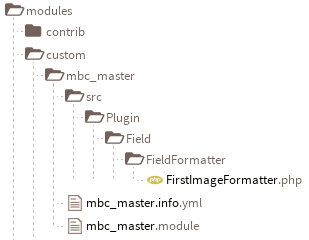
\includegraphics{mbc_master}
  \caption{Esquema de pastas e arquivos do módulo MBC Master.}
  \label{mbc_master}
\end{figure}

% =========================================================================== %
\subsection{Módulo 2 - MBC Review}
Este módulo foi criado com o objetivo de prover um método para o administrador do site enviar e-mail para usuários pedindo Reviews de produtos ou Opiniões sobre a empresa, prover um link exclusivo para criação destes conteúdos que vai neste e-mail, que reconhece automaticamente o usuário e não publique este conteúdo, deixando-o para moderação do administrador.

% =========================================================================== %
\subsection{Módulo Adaptado - TinyPNG}
Por ser um módulo bem simples que utiliza uma biblioteca externa para fazer a minificação, a adptação deste módulo foi bem simples. Uma função que é executada quando uma entidade (conteúdo) é salva foi utilizada e usada a biblioteca tinify \url{http://packagist.org/packages/tinify/tinify} para executar a minificação das imagens. Além disso, o módulo adiciona uma página administrativa para ser gerenciada a chave da API do serviço, que pode ser obtida no site \url{https://tinypng.com/}.

% =========================================================================== %
\subsection{Sub-tema - MBC Theme}
Todo front-end do site é construido neste sub-tema. A base é o framework Bootstrap e seu tema para Drupal 8. 

\subsubsection{Gulp}
O automatizador de tarefas Gulp foi utilizado para algumas das principais tarefas de desenvolvimento deste tema como descrito anteriormente e o resultado foi um fluxo de front-end bem mais rápido, sólido e seguro. Todas as ferramentas funcionaram como previsto e todo o código de LESS e Javascript que foram necessários, seguem um padrão de código bem definido e não possuem estruturas inseguras.

\subsubsection{LESS}
Para os arquivos Less, que vão gerar o CSS do site, utilizamos uma estrutura modular, onde cada bloco e página do site tem seu próprio LESS, resultando em arquivos com menos 100 linhas, de facil manutenção e preparados para melhorias no carregamento do CSS pelas páginas do site.

\begin{figure}[ht]
  \centering
  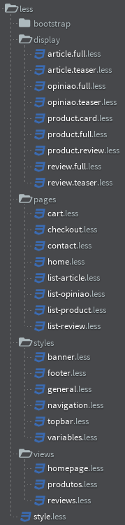
\includegraphics{less}
  \caption{Exemplo de arquivo LESS e sua estrutura de pastas e arquivos.}
  \label{less}
\end{figure}

\subsubsection{Templates Twig}
O Drupal 8 tem um sistema de templates que são utilizados para montar as páginas. Para customizar estes templates, temos que sobrescrevê-los. Nosso tema base já possui vários templates sobrescritos do núcleo e nós nos baseamos nestes para fazer os nossos. Até o momento foram necessários mais de 20 templates e com as melhorias sendo feitas constantemente no site, mais serão criados.

\begin{figure}[ht]
  \centering
  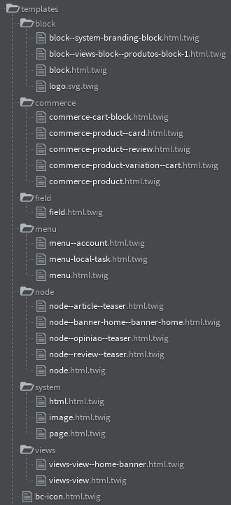
\includegraphics{templates}
  \caption{Exemplo de arquivo TWIG de template e sua estrutura de pastas e arquivos.}
  \label{templates}
\end{figure}

% @@@@@@@@@@@@@@@@@@@@@@@@@@@@@@@@@@@@@@@@@@@@@@@@@@@@@@@@@@@@@@@@@@@@@@@@@@@ %
% @@@@@@@@@@@@@@@@@@@@@@@@@@@@@@@@@@@@@@@@@@@@@@@@@@@@@@@@@@@@@@@@@@@@@@@@@@@ %
\section{Performance}

Medimos a performance do site pelo serviço previamente apresentado chamado GTMetrix. As notas obtidas são bem constantes a cada análise, porém o tempo de resposta do servidor pode mudar significativamente a cada requisição. Configuramos a ferramenta para utilizar um servidor brasileiro, mais especificamente em São Paulo para ser fiel ao público alvo do site e utilizar o browser Google Chrome, o mais utilizado com 76.87\%\cite{Chrome} dos usuários.

% =========================================================================== %
\subsection{Tempo de Carregamento}

\begin{figure}[ht]
  \centering
  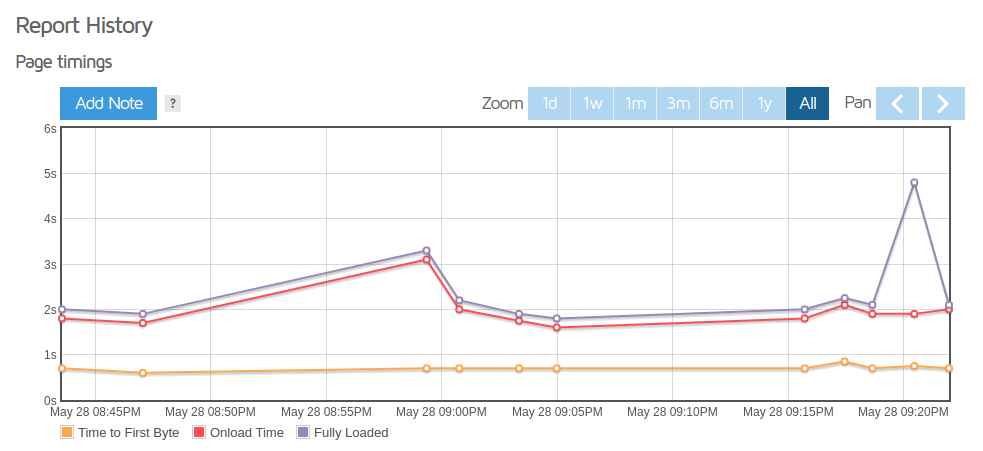
\includegraphics{gtmetrix_history}
  \caption{Gráfico de tempos de carregamento da página na ferramenta GTMetrix.}
  \label{gtmetrix_history}
\end{figure}

Vemos na imagem acima\ref{gtmetrix_history}, os tempos de carregamento do site representados pela linha vermelha, tem uma média de 2 segundos. Em apenas um caso este tempo ficou perto dos 3 segundos e em outro, o tempo de carregamento total, que é quando todo o Javascript da página terminou sua execução, foi de aproximados 5 segundo. O tempo entre a requisição da página e o retorno do servidor ficou sempre abaixo do 1 segundo como podemos ver no gráfico pela linha amarela.

% =========================================================================== %
\subsection{Nota, PageSize & Total de Requests}

\begin{figure}[ht]
  \centering
  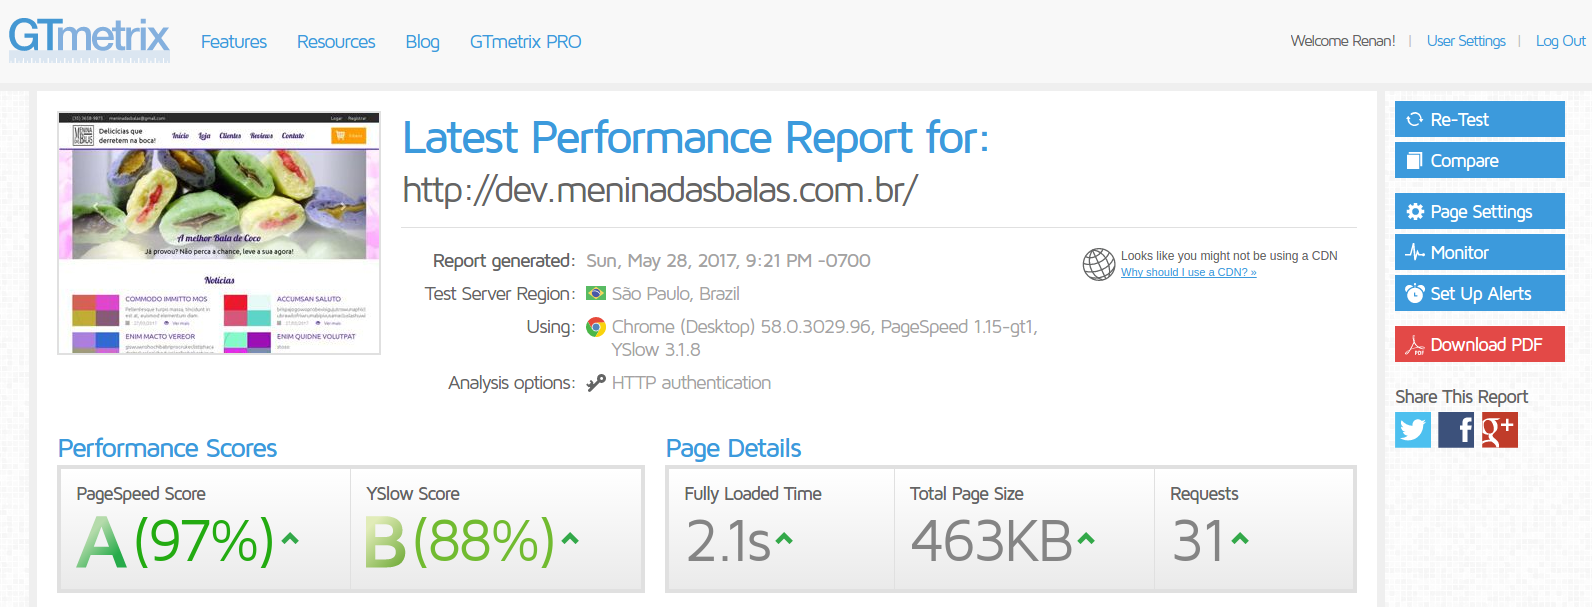
\includegraphics{gtmetrix}
  \caption{Resultado geral de desempenho do site em ambiênte de desenvolvimento na ferramenta GTMetrix.}
  \label{gtmetrix}
\end{figure}

Acima\ref{gtmetrix} vemos o resultado geral do site na ferramenta GTMetrix. Uma nota excelente foi alcançada no PageSpeed, atingindo 97\% e no YSlow a nota foi boa, chegando a 88\%. Mais adiante veremos o que faltou para estas notas atingirem o 100\%. O tamanho da página também ficou bom, pois a própria ferramenta diz que a média geral é de 2.52MB e nós conseguimos uma homepage com menos de 0.5MB. Outra informação dada é o número de requests, atingindo 31, com a média geral do GTMetrix sendo 85.

% =========================================================================== %
\subsection{PageSpeed}

\begin{figure}[ht]
  \centering
  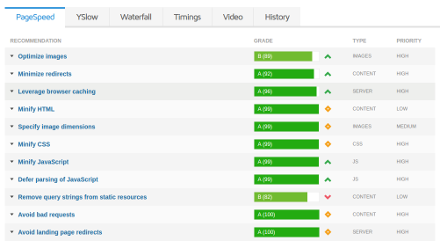
\includegraphics{gtmetrix_pagespeed}
  \caption{Pontos a melhorar dados pela ferramenta GTMetrix, ordenadas por relevância, fornecidos pelo PageSpeed.}
  \label{gtmetrix_pagespeed}
\end{figure}

Vamos agora analisar as notas abaixo da nossa média dada pelo PageSpeed e suas dicas para melhorar.

\subsubsection{Optimize Images}
Apesar de já utilizarmos uma ferramenta para minificação das imagens, não foi suficiente para alcançar-mos a melhor nota. A ferramenta acusa que algumas imagens podem ser minificadas ainda mais, entre 3\% e 10\%. Resolvemos não fazer esta melhoria, pois a ferramenta atual já funciona bem e a diferença na nota não compensaria o trabalho.

\subsubsection{Minimize Redirects}
Neste quesito, fomos penalizados na nota pois o recurso de Javascript do Google Analytics, adicionado pelo módulo Drupal, é requerido pelo protocolo HTTP e um redirecionamento é feito pelo Google para HTTPS. A diferença dos dois é uma encriptação que aumenta a segurança. Este problema nós só conseguiremos resolver mudando nosso protocolo para HTTPS também, algo que esta na lista de melhorias futuras.

\subsubsection{Leverage browser caching}
Esta é outra penalização por conta do Google Analytics. O mesmo recurso Javascript do item anterior, que é necessário para a ferramenta funcionar, retorna com um header de cache de apenas 2 horas, considerado pouco pelo GTMetrix. Uma solução seria baixar este arquivo e servi-lo do nosso domínio com um cache melhor, porém isso pode prejudicar o uso do Analytics por este ser atualizado constantemente. Assim, escolhemos deixar esta nota como está.

\subsubsection{Remove query strings from static resources}
Os recursos do nosso site, imagens, css e javascript são servidos pelo Drupal e este, utiliza query strings nas urls para controle de cache. Remover estes removeria este controle do sistema sobre os arquivos cacheados, piorando o desempenho em geral. Por este motivo, esta dica também será ignorada.

% =========================================================================== %
\subsection{YSlow}

Agora, analisaremos as dicas da ferramenta YSlow.

\begin{figure}[ht]
  \centering
  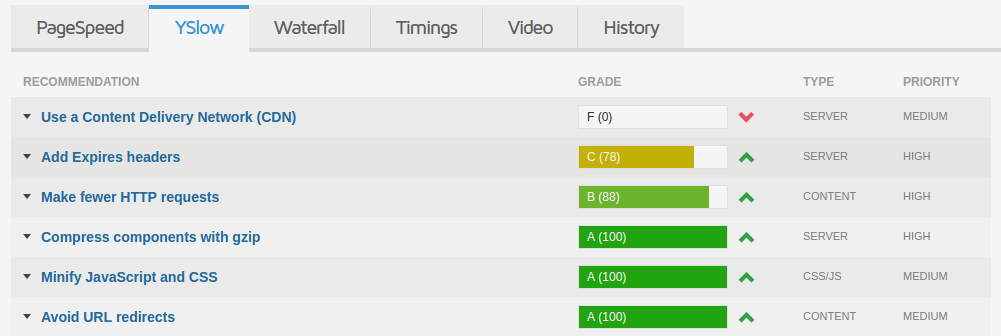
\includegraphics{gtmetrix_yslow}
  \caption{Pontos a melhorar dados pela ferramenta GTMetrix, ordenadas por relevância, fornecidos pelo YSlow.}
  \label{gtmetrix_yslow}
\end{figure}

\subsubsection{Use a Content Delivery Network}
Neste item, é sugerido que utilizemos um CDN (Rede Central de Distribuição) para servir os arquivos estáticos do site, como CSS, javascript e imagens. Em um CDN, os arquivos ficariam em vários servidores de diferentes localizações e quando uma requisição fosse feita, o servidor mais próximo ou com melhor capacidade seria o escolhido para servir estes arquivos, fazendo com que a velocidade de um site aumente consideravelmente. Por ter um custo alto, este recurso só deve ser implementado em sites muito grandes com milhões de acessos diários. Porque nosso site não ter a pretenção de ter um número tão alto de acessos e também por fugir do orçamento do cliente, esta melhoria não será implementada.

\subsubsection{Add expire headers}
Assim como o PageSpeed, o YSlow penaliza por header de cache com tempo de expiração curto. Desta vez dois recursos externos foram citados, o javascript do Google Analytics e o css de fontes do Google Fonts. Novamente, por serem recursos externos, não temos controle sobre o header e deixaremos esta dica sem ação.

\subsubsection{Make fewer HTTP requests}
Esta dica aparece porque o nosso CSS e Javascript foram agregados e separados em 4 arquivos cada. Segundo o YSlow, poderiamos agregar ainda mais e diminuir para um arquivo de cada tipo. Isto não pode ser feito no CSS por que o arquivo não pode ter mais que um número específico de seletores, para manter o suporte ao browser Internet Explorer em versões abaixo do 9. No javascript o problema é o módulo que faz a agregação, que não permite menos de 4 arquivos, que é o considerado ideal pelo criador \cite{AdvAgg}.

% @@@@@@@@@@@@@@@@@@@@@@@@@@@@@@@@@@@@@@@@@@@@@@@@@@@@@@@@@@@@@@@@@@@@@@@@@@@ %
% @@@@@@@@@@@@@@@@@@@@@@@@@@@@@@@@@@@@@@@@@@@@@@@@@@@@@@@@@@@@@@@@@@@@@@@@@@@ %
\section{E-commerce}
O módulo Commerce do Drupal fez todo o trabalho pesado para a construção de um e-commerce. Só resta ao desenvolvedor fazer as configurações, criar campos e customizar o que for preciso. Tudo isto é feito guiado pelas instruções do módulo.

A dificuldade do projeto está focada em duas questões do e-commerce, o método de envio e o método de pagamento. O envio no Brasil é feito pelos Correios, que oferece uma API para consulta de preços. Porem, não temos ainda um módulo que faça esta integração e o desenvolvimento deste daria um trabalho de conclusão por si só. O mesmo acontece com o método de pagamento, as opções nacionais não estão implementadas, nos deixando com os serviços globais, como o que utilizamos, o PayPal.

No front-end, vários templates e muito CSS ajudam a melhorar o estilo das páginas, que não possuem um tema \textit{'out-of-the-box'}. Tudo isso fez com que o resultado final seja um e-commerce simples, porém robusto e que se trabalhado mais algum tempo, tem um grande potencial.

% @@@@@@@@@@@@@@@@@@@@@@@@@@@@@@@@@@@@@@@@@@@@@@@@@@@@@@@@@@@@@@@@@@@@@@@@@@@ %
% @@@@@@@@@@@@@@@@@@@@@@@@@@@@@@@@@@@@@@@@@@@@@@@@@@@@@@@@@@@@@@@@@@@@@@@@@@@ %
\section{Final}

O resultado final pode ser verificado nas imagens no apêndice \ref{appendix:Site} ou no próprio site no endereço:

\begin{center}
  \url{https://meninadasbalas.com.br/}
\end{center}

Todo o código feito pode ser visto e baixado no repositório público do projeto no Github no endereço:

\begin{center}
  \url{https://github.com/renanmfd/meninadasbalas}
\end{center}

